\documentclass{beamer}
%
% Choose how your presentation looks.
%
% For more themes, color themes and font themes, see:
% http://deic.uab.es/~iblanes/beamer_gallery/index_by_theme.html
%
\mode<presentation>
{
  \usetheme{Madrid}      % or try Darmstadt, Madrid, Warsaw, ...
  \usecolortheme{beaver} % or try albatross, beaver, crane, ...
  \usefonttheme{serif}  % or try serif, structurebold, ...
  \setbeamertemplate{navigation symbols}{}
  \setbeamertemplate{caption}[numbered]
} 

\usepackage{hyperref}
\usepackage{tabu}
\usepackage[italian]{babel}
\usepackage[utf8]{inputenc}
\usepackage{pdfpages}
\usepackage{framed, color}
\definecolor{shadecolor}{rgb}{1,0.8,0.3}
\usepackage{color}
\usepackage[backend=bibtex, style=numeric,sorting=none]{biblatex}

\definecolor{pblue}{rgb}{0.13,0.13,1}
\definecolor{pgreen}{rgb}{0,0.5,0}
\definecolor{pred}{rgb}{0.9,0,0}
\definecolor{pgrey}{rgb}{0.46,0.45,0.48}

\usepackage{listings}
\lstset{language=Python,
  showspaces=false,
  showtabs=false,
  breaklines=true,
  showstringspaces=false,
  breakatwhitespace=true,
  commentstyle=\color{pgreen},
  keywordstyle=\color{pblue},
  stringstyle=\color{pred},
  basicstyle=\ttfamily,
  frame=lrbt,xleftmargin=\fboxsep,xrightmargin=-\fboxsep
}

\title[Ragazze Digitali 2019]{Ragazze Digitali A.A. 2018/2019}
\author{E. Salvucci - S. Gattucci - C. Varini}
\date{}

\AtBeginSection[]
{
  \begin{frame}<beamer>
    \frametitle{Outline}
    \tableofcontents[currentsection,currentsubsection]
  \end{frame}
}

\bibstyle{unsrt}
\bibliography{bibliography.bib}

\begin{document}

\setbeamertemplate{background}
{
\includegraphics[width=\paperwidth,height=\paperheight]{images/ragazze_digitali.jpg}}
\begin{frame}
\end{frame}

\setbeamertemplate{background}{}

\begin{frame}{Cosa faremo oggi}
\texttt{Ti trovi in una terra piena di draghi.\newline
        Di fronte a te ci sono due grotte\newline
        In una grotta si trova un drago simpatico e socievole che condividerà con te il suo tesoro.\newline
        Nell'altra grotta c'è invece un drago affamato e vorace.\newline
        Dentro quale grotta vuoi entrare? (1 o 2)\newline}
\textbf{1\newline}
\texttt{Entri nella caverna 1\newline
        E' buia e spaventosa\newline
        Un enorme drago compare all'improvviso davanti a te! Apre le sue fauci e... ti inghiottisce in un batter d'occhio!\newline
        Vuoi giocare ancora?\newline}
\textbf{No}        
        
\end{frame}

\section{Funzioni}

\begin{frame}[fragile]
\frametitle{Funzioni}
    \begin{block}{}
        \begin{itemize}
            \item Abbiamo già visto e usato alcune funzioni, ad esempio: print('ciao'), input(), randint(1, 20), ecc..
            \item Possiamo anche crearne noi!
            \item Con le funzioni possiamo incapsulare del codice e riutilizzarlo più volte nel nostro programma.
        \end{itemize}
    \end{block}
    
    \begin{block}{Una funzione}
        \begin{itemize}
            \item Deve essere dichiarata \textbf{prima} di essere chiamata
            \item Può avere dei parametri
            \item Restituisce un risultato
        \end{itemize}
    \end{block}
\end{frame}

\begin{frame}[fragile]
\frametitle{Funzioni}
        \begin{block}{Come si dichiara una funzione}
            \begin{itemize}
                \item Utilizziamo la keyword \textbf{def}
                \item seguita dal \textbf{nome} della funzione
                \item Seguita dai \textbf{parametri} racchiusi tra parentesi (o le sole parentesi aperta e chiusa nel caso non ci siano parametri)
                \item Seguiti da \textbf{:}
            \end{itemize}
        \end{block}

        \begin{columns}
	    \begin{column}{4cm}
			\begin{figure}
   				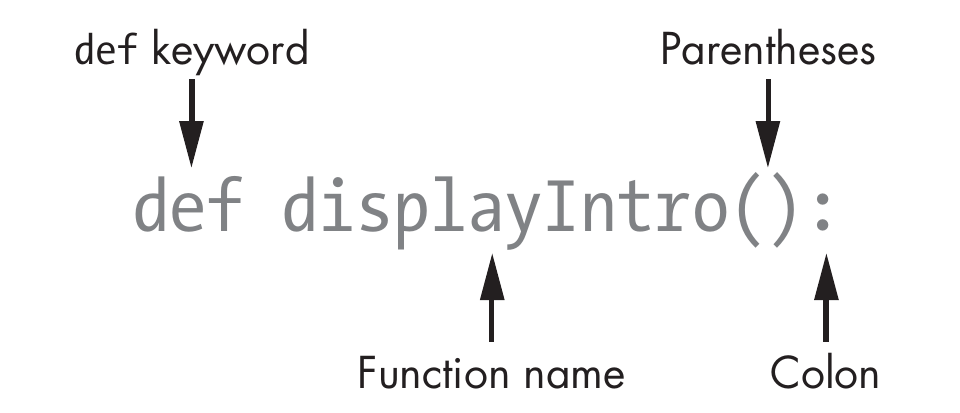
\includegraphics[height=2cm]{images/function_signature_example.png}
			\end{figure}
		\end{column}
		
		\begin{column}{6cm}
            \begin{lstlisting}
def displayIntro():
    print('''Ti trovi in una terra piena di draghi...''')
    print()
            \end{lstlisting}
		\end{column}
	\end{columns}
	! notiamo il print(''' '''), stringa multilinea
\end{frame}

\begin{frame}
\frametitle{Funzioni}
    \begin{block}{Alcuni consigli..}
        \begin{itemize}
            \item Ciò che abbiamo detto per i nomi delle variabili vale anche per i nomi delle funzioni
            \item Meglio se le nostre funzioni sono corte, con poco codice
            \item  Con 1 funzione facciamo 1 cosa soltanto!
            \item Evitiamo di usare più di 1 o 2 parametri in una funzione
            
            Se abbiamo bisogno di più parametri dividiamo quello che vogliamo fare in più funzioni
        \end{itemize}
    \end{block}
\end{frame}

\begin{frame}[fragile]
\frametitle{Funzioni}
    \begin{block}{Funzioni con parametri}
        \begin{itemize}
            \item Possiamo "dare in pasto" ad una funzione dei dati, delle informazioni, che chiamiamo \textbf{parametri}
            \item Queste informazioni ci serviranno per elaborare il risultato della funzione
        \end{itemize}
    \end{block}
    
    \begin{lstlisting}
                          # O ancora meglio..
def isPositive(number): | def isPositive(number): 
    if number > 0 :     |    return number > 0
        return True     |
    else:               |
        return False    |
    \end{lstlisting}
    
    \begin{lstlisting}
# Usiamo la funzione, ad esempio, in questo modo
print(isPositive(5))    # True
print(isPositive(-5))   # False
    \end{lstlisting}
    
\end{frame}

\begin{frame}[fragile]
\frametitle{Funzioni}
    \begin{block}{Funzioni con parametri}
        \begin{itemize}
            \item Possiamo "dare in pasto" ad una funzione dei dati, delle informazioni, che chiamiamo \textbf{parametri}
            \item Queste informazioni ci serviranno per elaborare il risultato della funzione
            \item Il risultato verrà restituito utilizzando la keyword \textbf{return}
        \end{itemize}
    \end{block}
    
    \begin{lstlisting}
def sum(firstNumber, secondNumber): 
    return firstNumber + secondNumber
    \end{lstlisting}
    
    \begin{lstlisting}
# Usiamo la funzione, ad esempio, in questo modo
result = sum(5, 4)    # result avra' valore 9
result = sum(-10, 5)  # result avra' valore -5
    \end{lstlisting}
    
\end{frame}

\section{Variabili locali e variabili globali}

\begin{frame}[fragile]
\frametitle{Variabili locali e variabili globali}
    \begin{block}{Variabili locali}
        Chiamiamo \textbf{Variabile locale} qualunque variabile dichiarata all'interno di una funzione, questa esiste solo all'interno della funzione stessa
        
        Le variabili locali vengono "dimenticate" dopo che la funzione ha raggiunto il return (e quindi ha finito le sue elaborazioni)
    \end{block}
    
    \begin{lstlisting}
def welcomePerson():
    person = 'Chiara'     # Variablile locale
    print('Benvenuta ' + person)
# Anche se non c'e' il return, da qui in poi la variable non ha piu' effetto
    \end{lstlisting}
    
    \begin{lstlisting}
welcomePerson()
person = 'Sofia'
print(person) # Sofia
welcomePerson() # Benvenuta Chiara
    \end{lstlisting}
\end{frame}

\begin{frame}[fragile]
\frametitle{Variabili globali}
    \begin{block}{Variabili globali}
        Nell'esempio precedente person = 'Sofia' e' una variabile globale, ovvero una variabile che ha effetto in tutto il nostro programma
        
        Modifichiamo leggermente l'esempio:
    \end{block}
    
        \begin{lstlisting}
def welcomePerson():
    print('Benvenuta ' + person)
    \end{lstlisting}
    
    \begin{lstlisting}
person = 'Chiara'     # Variablile globale
welcomePerson() # Benvenuta Chiara
person = 'Sofia'
welcomePerson() # Benvenuta Sofia
    \end{lstlisting}
\end{frame}

\section{Operatori booleani}

\begin{frame}[fragile]
\frametitle{Operatore and (e)}
\begin{block}{Quale frase è complessivamente vera e quale falsa?}
    \begin{itemize}
        \item I gatti hanno i baffi E i cani hanno la coda
        \item I gatti hanno i baffi E i cani hanno le ali
        \item I gatti abbaiano E i cani hanno le ali
    \end{itemize}
\end{block}

\end{frame}

\begin{frame}[fragile]
\frametitle{Operatore and (e)}

\begin{tabu} to 0.8\textwidth { | X[l] | X[c] | X[c] |  X[r] |}
 \hline
  & & & Risultato\\
 \hline
 True & \textbf{and} & True & True\\
 \hline
 True & \textbf{and} & False & False\\
 \hline
 False & \textbf{and} & True & False\\
\hline
 False & \textbf{and} & False& False\\
\hline
\end{tabu}

\end{frame}

\begin{frame}[fragile]
\frametitle{Operatore or (o)}
\begin{block}{Quale frase è complessivamente vera e quale falsa?}
    \begin{itemize}
        \item I gatti hanno i baffi O i cani hanno la coda
        \item I gatti hanno i baffi O i cani hanno le ali
        \item I gatti abbaiano O i cani hanno le ali
    \end{itemize}
\end{block}

    \begin{lstlisting}
city = 'Cesena'
result = 10 < 20 or city == 'Cesena'
# result avra' valore?
result = 10 > 20 or city == 'Cesena'
# result avra' valore?
    \end{lstlisting}

\end{frame}

\begin{frame}[fragile]
\frametitle{Operatore or (o)}

\begin{tabu} to 0.8\textwidth { | X[l] | X[c] | X[c] |  X[r] |}
 \hline
  & & & Risultato\\
 \hline
 True & \textbf{or} & True & True\\
 \hline
 True & \textbf{or} & False & True\\
 \hline
 False & \textbf{or} & True & True\\
\hline
 False & \textbf{or} & False& False\\
\hline
\end{tabu}

\end{frame}

\begin{frame}[fragile]
\frametitle{Operatore not}
    \begin{lstlisting}
city = 'Cesena'
result = not (10 < 20 or city == 'Cesena')
# result avra' valore?
result = not (10 > 20 or city == 'Cesena')
# result avra' valore?
    \end{lstlisting}

\end{frame}

\begin{frame}[fragile]
\frametitle{Operatore not}

\begin{tabu} to 0.8\textwidth { | X[c] |  X[c] |}
 \hline
  & Risultato\\
 \hline
 not True & False\\
 \hline
 not False & True\\
\hline
\end{tabu}

\end{frame}

\section{Costrutto while}

\begin{frame}[fragile]
\frametitle{Costrutto while}
\begin{block}{while}
    \begin{itemize}
        \item Costrutto simile al for, che abbiamo gia' visto
        \item Il while ripete il ciclo finche' una determinata condizone rimane vera 
        \item Qual e' la differenza con il for?
    \end{itemize}
\end{block}

    \begin{lstlisting}
while month == 'giugno' and year == '2019' :
    codice del ciclo while
    \end{lstlisting}
    
! come nel for, nell'if e nelle funzini occhio all'indentazione del codice del ciclo!

\end{frame}

\section{Variabili Costanti}

\begin{frame}[fragile]
\frametitle{Variabili Costanti}
    \begin{block}{Variabili costanti}
Capitera' di usare variabili il cui valore rimane costante nel tempo e che non verranno modificate dopo la loro prima dichiarazione.

Secondo la convenzione il nome di queste variabili va scritto tutto in maiuscolo e, se composto da piu parole, queste sono separate da \textunderscore (underscore).
    \end{block}
    
    \begin{lstlisting}
MAX_SIZE = 10
MIN_SIZE = 1
LENGHT = 10
POSITIVE_ANSWER = 'Si'# 
NEGATIVE_ANSWER = 'No' # Tra poco vedremo come gestire in modo piu' elegante i valori si/no
    \end{lstlisting}

\end{frame}

\section{Liste}

\begin{frame}[fragile]
\frametitle{Liste}
    \begin{block}{Liste}
Le liste sono delle variabili che, invece che contenere dei singoli valori ne contengono molteplici.
    \end{block}
    
    \begin{lstlisting}
teachers =  ['Chiara', 'Enrico', 'Sofia']
answers = ['Si', 'No']
vocals = ['a', 'e', 'i', 'o', 'u']
    \end{lstlisting}
\end{frame}

\begin{frame}[fragile]
\frametitle{Liste}
    \begin{block}{Come leggiamo i valori di una lista}
Pensiamo ad una lista come ad un mobile con dei cassetti numerati da 0 (primo cassetto) a lungezza della lista -1 (ultimo cassetto).

! Attenzione, stiamo partendo da 0 !
    \end{block}
    
    \begin{lstlisting}
vocals = ['a', 'e', 'i', 'o', 'u']
    \end{lstlisting}
    
        \begin{block}{}
Per aprire i "cassetti" e leggere i singoli valori della lista quindi faremo
    \end{block}

    \begin{lstlisting}
vocals[0] # Avra' valore 'a'
vocals[1] # Avra' valore 'e'
vocals[2] # ...
vocals[3]
vocals[4]
    \end{lstlisting}

\end{frame}

\begin{frame}[fragile]
\frametitle{Liste}
    \begin{block}{Come scriviamo i valori di una lista}
Similmente a come li leggiamo e a come assegnamo un valore ad una variabile normale.
    \end{block}
    
    \begin{lstlisting}
answers = ['Si', 'No']

answers[0] = 'Yes' # Nella posizione 0 della lista scrivo 'Yes', sostituendolo al 'Si'
    \end{lstlisting}

    \begin{block}{append()}
La funzione append() aggiunge valori ad una lista gia' definita
    \end{block}

    \begin{lstlisting}
answers = ['Si', 'No']

answers.append('Forse') # Ora answers avra' valori ['Si', 'No', 'Forse']
    \end{lstlisting}

\end{frame}

\begin{frame}[fragile]
\frametitle{Liste}
    \begin{block}{reverse()}
La funzione reverse() inverte l'ordine degli elementi di una lista, modificando la lita stessa!

! Si, la lista e' ordinata !
    \end{block}

    \begin{lstlisting}
vocals = ['a', 'e', 'i', 'o', 'u']
vocals.reverse() # ['u', 'o', 'i', 'e', 'a']
    \end{lstlisting}

\end{frame}

\begin{frame}[fragile]
\frametitle{Liste}
    \begin{block}{Lista vuota}
Adesso che conosciamo append() possiamo anche crearci delle lista vuote e all'occorrenza aggiungere valori
    \end{block}
    
    \begin{lstlisting}
answers = []
answers.append('Si')
answers.append('No')
    \end{lstlisting}

    \begin{block}{Lista piena}
Utilizzando la funzione remove() possiamo rimuovere dei valori
    \end{block}
    
    \begin{lstlisting}
days = [10, 11, 12, 13, 14]
days.remove(12)
print(days) # [10, 11, 13, 14]
    \end{lstlisting}

    \begin{block}{reverse()}
La funzione reverse() inverte l'ordine degli elementi di una lista, modificando la lita stessa!

! Si, la lista e' ordinata !
    \end{block}

    \begin{lstlisting}
vocals = ['a', 'e', 'i', 'o', 'u']
vocals.reverse() # ['u', 'o', 'i', 'e', 'a']
    \end{lstlisting}

\end{frame}


\begin{frame}[fragile]
\frametitle{Liste}
    \begin{block}{split()}
Un'altra funzione utile e' split().
Data una frase, un insieme di parole separate da spazi, split() restituisce una lista fatta dalle parole della frase stessa
    \end{block}
    
    \begin{lstlisting}
sentence = 'Oggi a Cesena nevica e fa un gran caldo'
sentence.split()
# ['Oggi', 'a', 'Cesena', 'nevica', 'e', 'fa', 'un', 'gran', 'caldo']
splittedSentence = sentence.split()
splittedSentence[3] # Quale valore avra'?
    \end{lstlisting}

\end{frame}

\begin{frame}[fragile]
\frametitle{Liste}
    \begin{block}{Cosa succede se...}
provo a leggere in una posizione maggiore della lunghezza della lista?
    \end{block}
    
    \begin{lstlisting}
vocals = ['a', 'e', 'i', 'o', 'u']
print(vocals[999])
print(vocals[10])
    \end{lstlisting}

\end{frame}

\begin{frame}[fragile]
\frametitle{Liste}
    \begin{block}{Cosa succede se...}
provo a leggere o scrivere in una posizione maggiore della lunghezza della lista?
    \end{block}
    
    \begin{lstlisting}
vocals = ['a', 'e', 'i', 'o', 'u']
print(vocals[999])
'vocals[9999]
IndexError: list index out of range'

vocals[10] = 'abcdefghi...'
'IndexError: list assignment index out of range'
    \end{lstlisting}
\end{frame}

\begin{frame}[fragile]
\frametitle{Liste}
    \begin{block}{range()}
    La funzione range restituisce una lista di numeri interi compresi nell'intervallo specificato come parametro
    \end{block}
    
    \begin{lstlisting}
range(5) # [0, 1, 2, 3, 4]
# Se non specifico il minimo parto da 0    
range(0, 10) # [0, 1, 2, 3, 4, 5, 6, 7, 8, 9]
range(5, 10) # [5, 6, 7, 8, 9] ! Il 10 non c'e'
    \end{lstlisting}
\end{frame}

\begin{frame}[fragile]
\frametitle{Liste}
    \begin{block}{list()}
    La funzione list prende come parametro un valore e restituisce una lista fatta degli elementi che compongono il parametro
    \end{block}
    
    \begin{lstlisting}
list('Ciao') # ['C', 'i', 'a', 'o']
    \end{lstlisting}
\end{frame}

\begin{frame}[fragile]
\frametitle{Liste}
    \begin{block}{Operatore in}
    L'operatore \textbf{in} ci dice se un determinato elemento sia contenuto in una lista o meno.
    \end{block}
    
    \begin{lstlisting}
    vocals = ['a', 'e', 'i', 'o', 'u']
    'e' in vocals # ???
    'g' in vocals # ???
    \end{lstlisting}
\end{frame}

\begin{frame}[fragile]
\frametitle{Liste}
    \begin{block}{len(vocals)}
    La funzione \textbf{len(vocals)} la lunghezza della lista di nome vocals.
    \end{block}
    
    \begin{lstlisting}
    vocals = ['a', 'e', 'i', 'o', 'u']
    len(vocals) # ???
    \end{lstlisting}
\end{frame}



\section{L'impiccato}

\begin{frame}
\frametitle{L'impiccato - Parte 0}
    Per realizzare il gioco dell'impiccato dovrete completare il codice che trovate a questo
\href{https://raw.githubusercontent.com/ragazzedigitalicesena/slide-2019/master/tex/chapter_5-8/hangman.py}{link} seguendo le indicazioni riportate nelle pagine successive

\vspace{5mm}
\href{https://raw.githubusercontent.com/ragazzedigitalicesena/slide-2019/master/tex/chapter_5-8/hangman.py}{Download}
\end{frame}

\begin{frame}[fragile]
\frametitle{L'impiccato - Parte 1}

\begin{block}{E' il vostro turno!}
    
    \begin{itemize}
        \item Importa il modulo random, come visto in precedenza
        \item Crea una variabile globale chiamata words (nello specifico una stringa) che contenga le parole che il giocatore dovra' indovinare separate da spazi. Trasforma quindi la stringa in una lista che abbia le parole della variabile creata come elementi [aiuto: utilizza la funzione split()]
        \item Crea una variabile globale chiamata missedLetters (una stringa vuota nello specifico) con la quale memorizzeremo le lettere sbagliate inserite dall'utente
        \item Crea una variabile globale chiamata correctLetters (una stringa vuota nello specifico) on la quale memorizzeremo le lettere sbagliate inserite dall'utente
        \item Crea una variabile globale chiamamta secretWord il cui valore e' il risultato della funzione che ritorna una parola casuale dalla lista di parole
    \end{itemize}
\end{block}
\end{frame}

\begin{frame}[fragile]
\frametitle{L'impiccato - Parte 2}

\begin{block}{E' il vostro turno!}

    \begin{itemize}
        \item Crea una funzione chiamata getRandomWord(wordList) che, data come parametro una lista di parole (la quale in precedenza abbiamo chiamato words), restituisca un suo elemento random
        
        (ad esempio se ho la lista ['Ragazze', 'Digitali', 'Cesena', 'Giugno'] mi deve restituire un elemento random di questa lista).
    \end{itemize}
\end{block}
\end{frame}

\begin{frame}[fragile]
\frametitle{L'impiccato - Parte 3}

\begin{block}{E' il vostro turno!}
Crea una funzione, dandole il nome che preferisci, che ci servira' per mostrare a video il 'campo di gioco'
In particolare la funzione dovra':
    \begin{itemize}
        \item Prendere come parametri la stringa contenente le lettere sbagliate inserite dal giocatore, la stringa contenente le lettere corrette inserite dal giocatore e la parola da indovinare
        \item Stampare a video l'immagine dell'impiccato corrispondente al numero di errori commessi, presa dalla lista HANGMAN\_PICS creata in precedenza, 
        
        Ad esempio: se il giocatore ha commesso 0 errori stampera' l'immagine alla posizione 0 della lista HANGMAN\_PICS, se ha commesso 1 errore stampera' l'immagine alla posizione 1 e cosi' via..
        \item Stampare a video tutte le lettere sbagliate inserite dal giocatore
    \end{itemize}
\end{block}

Vedi esempio alla pagina sucessiva
\end{frame}

\begin{frame}[fragile]
\frametitle{L'impiccato - Parte 3}

\begin{lstlisting}
  +---+
  O   |
 /|\  |
 / \  |
     ===

Lettere sbagliate: a b c d f h 
\end{lstlisting}

\end{frame}

\begin{frame}[fragile]
\frametitle{L'impiccato - Parte 4}

\begin{block}{E' il vostro turno!}
All'interno della funzione creata nella Parte 3 aggiungi
    \begin{itemize}
        \item una lista inizialmente vuota, dandole il nome che preferisci. Questa sara' una variabile locale della funzione nella quale scriveremo o le lettere inserite corretamente dal giocatore oppure dei '\_'
        \item un ciclo for che, per un numero di volte pari alla lunghezza della parola segreta da indovinare, aggiunga alla lista creata nel punto precedente o la lettera della parola segreta (se presente tra le lettere indovinate) oppure il carattere '\_' [aiuto: utilizza la funzione append('a')]
        
        Esempio: Se la parola da indovinare e' 'ciao' e ho inserito correttamente le lettere 'i o' il risultato dovra' essere ['\_', 'i', '\_', 'o']
        \item Stampa a video la lista appena creata e popolata dalle lettere corrette inserite oppure dai '\_'
    \end{itemize}
\end{block}
\end{frame}

\begin{frame}[fragile]
\frametitle{L'impiccato - Parte 5}

\begin{block}{E' il vostro turno!}
Crea una funzione, chiamandola playAgain(), che chieda all'utente se vuole giocare di nuovo e restituisca, con return, la risposta (similmente a come abbiamo visto in precedenza con l'esempio per chiedere il nome)
\end{block}
\end{frame}

\begin{frame}[fragile]
\frametitle{L'impiccato - Parte 6}

\begin{block}{Leggi la parte finale del codice fornito}
    \begin{itemize}
        \item Che cosa fa il while?
        \item A che cosa ci serve la variabile play?
        \item Che differenza c'e' con il while dentro alla funzione getGuess()?
    \end{itemize}
\end{block}
\end{frame}

\end{document}